\chapter{Statements}\label{ch:Statements}
\begin{chapter_resume}
Este capítulo contiene ejemplos sin explicacion de los distintos elementos que se pueden utilizar en esta plantilla de \LaTeX

\vspace{0.7cm}

La función de este capítulo no es explicar el uso ni el funcionamiento del código sino servir como referencia para poder copiar y pegar el código del elemento que se desee utilizar.
Es conveniente recordar que es útil tener un capítulo que incluya los principales elementos, ya que es útil para asegurar la correcta compilación de todos los paquetes. 
Es decir, incluye una referencia, un acrónimo y utiliza todos la mayoría de los paquetes por lo que nos permite chequear que el documento está correctamente diseñado.

\vspace{0.7cm}

Sin más, sólo recordar que para reproducir cualquier utilidad aquí mostrada no hay más que copiar el código fuente y pegarlo en el lugar deseado del documento.
\end{chapter_resume}
A continuación se muestran diferentes ejemplos para la inclusión de los principales elementos que se utilizarán a lo largo de la tesis: citas, acrónimos, símbolos, tablas, figuras y ecuaciones. Esta sección sólo incluye el código para incluir el elemento en cuestión, en el capítulo anterior se detalla cada elemento.
%\Blindtext

%\section{Tables}
%  \begin{enumerate}
%  \item Tabla:
%  
%  \textbackslash{}begin\{table\}[location]
% 
%  \textbackslash{}centering
%
%  \textbackslash{}begin\{tabular\}\{l \textbar{} c \textbar{} r\}
%
%  Label 1 \& Label 2 \& Label 3 \textbackslash{}\textbackslash{}
%
%  \textbackslash{}hline
%
%  1 \& 2 \& 3 \textbackslash{}\textbackslash{}
%
%  4 \& 5 \& 6 \textbackslash{}\textbackslash{}
%
%  7 \& 8 \& 9
%  
%  \textbackslash{}end\{tabular\}
%
%  \textbackslash{}caption\{Tabla simple\}
%
%  \textbackslash{}label\{tab:tablestatement\}
%
%  \textbackslash{}end\{table\}  
%
%  \begin{table}[ht]
%  \centering
%  \begin{tabular}{l | c | r}
%  Label 1 & Label 2 & Label 3 \\
%  \hline
%  1 & 2 & 3 \\
%  4 & 5 & 6 \\
%  7 & 8 & 9
%  \end{tabular}
%  \caption{Tabla simple}
%  \label{tab:tablestatement}
%  \end{table}
%\end{enumerate}
%\section{Figures}
%\begin{enumerate}
%  \item PNG/JPG/PDF:
%  
%  ``\textbackslash{}begin\{figure\}[location]
%  
%  \textbackslash{}centering
%  
%  \textbackslash{}includegraphics[options]\{Intro_TexMakerConf.png}
%
%  \textbackslash{}caption\{An example graph\}
%
%  \textbackslash{}label\{fig:x generalgraph\}
%
%  \textbackslash{}end\{figure\}''
%\begin{figure}[ht]
%\centering
%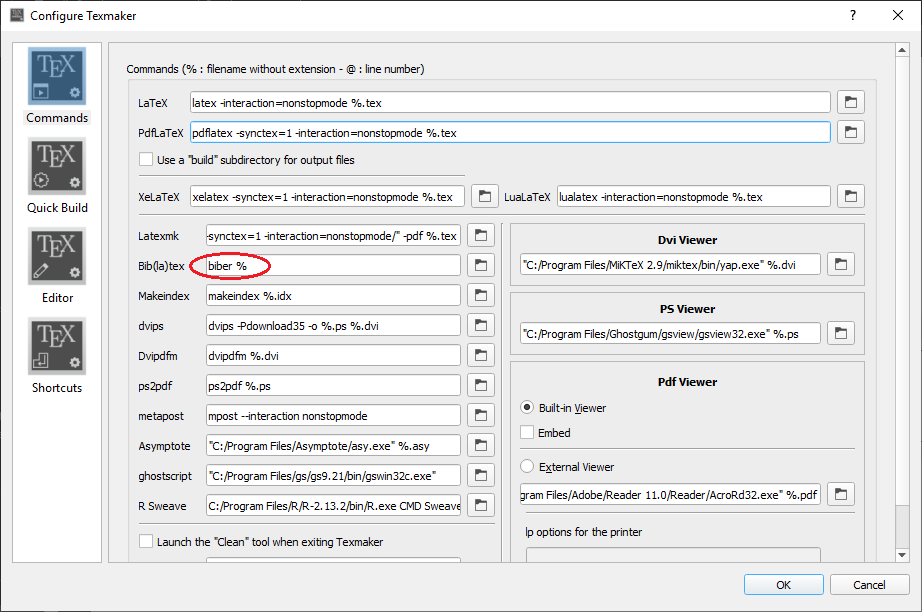
\includegraphics[scale=0.5]{Intro_TexMakerConf.png}
%\caption{PNG, JPG and PDF graph example}
%\label{fig:x generalgraph}
%\end{figure}
%  \item SVG:
%
%  ``\textbackslash{}begin\{figure\}[ht]
%  
%  \textbackslash{}centering
%
%  \textbackslash{}includesvg[options]\{svgimage\}
%
%  \textbackslash{}caption\{SVG graph statement example\}
%
%  \textbackslash{}label\{fig:x svgsatement\}
%
%  \textbackslash{}end\{figure\}''
%  \begin{figure}[ht]
%  \centering
%  \includesvg[scale=0.5]{svgimage}
%  \caption{SVG graph statement example}
%  \label{fig:x svgsatement}
%  \end{figure}
%\end{enumerate}
%\section{Lists}
%
%  \textbackslash{}begin\{enumerate\}
%  
%  \textbackslash{}setcounter\{enumi\}\{0\}
%
%  \textbackslash{}item Uno
%
%  \textbackslash{}item Dos
%
%  \textbackslash{}item Tres
%  
%  \textbackslash{}end\{enumerate\}
%
%\begin{enumerate}
%  \setcounter{enumi}{0}
%  \item Uno
%  \item Dos
%  \item Tres
%\end{enumerate}
%  
%  \textbackslash{}begin\{enumerate\}[font=\{\textbackslash{}color\{red!50!black\}\textbackslash{}bfseries\}]
%
%  \textbackslash{}setcounter\{enumi\}\{6\}
%
%  \textbackslash{}item Siete
%
%  \textbackslash{}item Ocho
%
%  \textbackslash{}item Nueve
%
%  \textbackslash{}end\{enumerate\}
%
%\begin{enumerate}[font={\color{red!50!black}\bfseries}]
%  \setcounter{enumi}{6}
%  \item Siete
%  \item Ocho
%  \item Nueve
%\end{enumerate}
%
%  \textbackslash{}begin\{itemize\}
%
%  \textbackslash{}item Item 1
%
%  \textbackslash{}item Item 2
%
%  \textbackslash{}item Item 3
%
%  \textbackslash{}end\{itemize\}
%  
%\begin{itemize}
%  \item Item 1
%  \item Item 2
%  \item Item 3
%\end{itemize}
%
%  \textbackslash{}begin\{enumerate\}[label=\{\textbackslash{}alph*\}]
%
%  \textbackslash{}item Item 1
%
%  \textbackslash{}item Item 2
%
%  \textbackslash{}item Item 3
%
%  \textbackslash{}end\{itemize\}
%  
%\begin{enumerate}[label={\alph*}]
%  %\setcounter{enumi}{6}
%  \item Item a
%  \item Item b
%  \item Item c
%\end{enumerate}
%
%  \textbackslash{}begin\{description\}
%
%  \textbackslash{}item [Volante] Controla la dirección de las ruedas
%
%  \textbackslash{}item [Acelerador] Controla la inyección de gasolina
%
%  \textbackslash{}item [Freno] Controla las pastillas de freno
%
%  \textbackslash{}end\{itemize\}
%  
%\begin{description}
%  \item [Volante] Controla la dirección de las ruedas
%  \item [Acelerador] Controla la inyección de gasolina
%  \item [Freno] Controla las pastillas de freno
%\end{description}
%
